% Appendices here
% \newgeometry{top=0.5cm,bottom=0.5cm}
\appendix
\addcontentsline{toc}{section}{Appendix}
\addtocontents{toc}{\protect\setcounter{tocdepth}{1}}
\section{Greyscale Comparison - Old Model A Learning Curves}
\subsection{Greyscale Applied To Gender \& Age Branches}
\begin{figure}[h!]
    \centering
    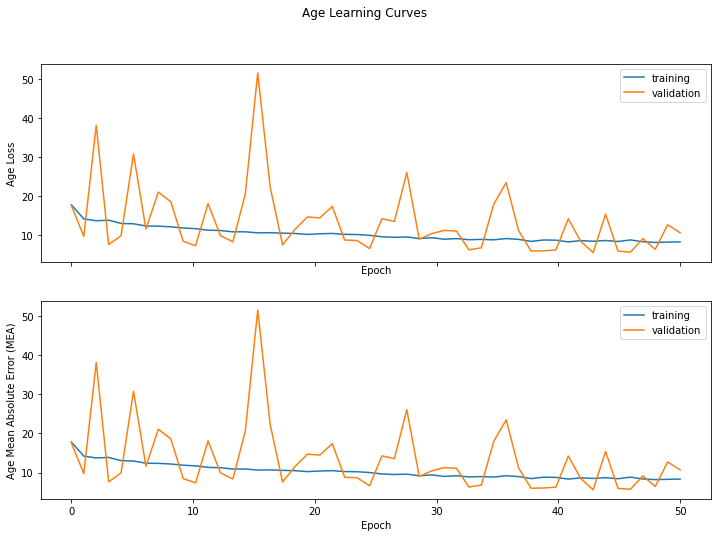
\includegraphics[height=0.42\textheight]{ModelA_AgeLearning_FCNDropout_BothGreyScale_NoRegularisation.png}
    \label{fig:modelA_gs_both_age_lc}
\end{figure}
\begin{figure}[h!]
    \centering
    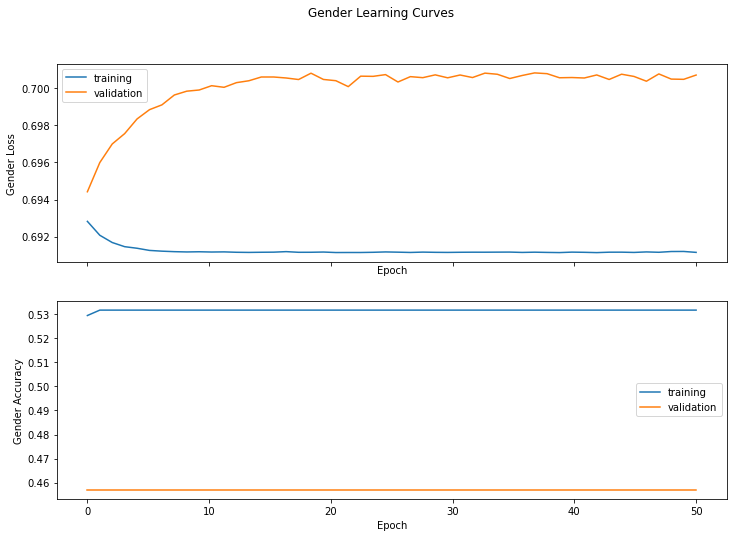
\includegraphics[height=0.42\textheight]{ModelA_GenderLearning_FCNDropout_BothGreyScale_NoRegularisation.png}
    \label{fig:modelA_gs_both_gender_lc}
\end{figure}
\newpage

\subsection{Greyscale Applied To Neither Branch}
\begin{figure}[h!]
    \centering
    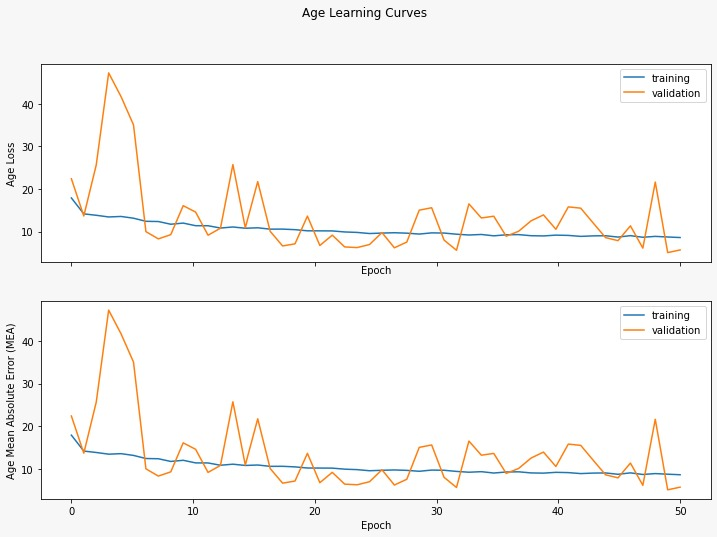
\includegraphics[height=0.42\textheight]{ModelA_AgeLearning_FCNDropout_NoGreyScale_NoRegularisation.jpeg}
    \label{fig:modelA_gs_neither_age_lc}
\end{figure}
\begin{figure}[h!]
    \centering
    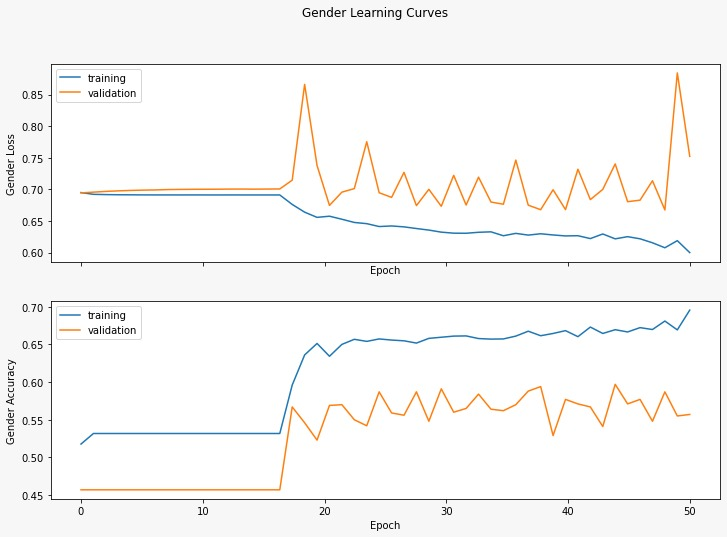
\includegraphics[height=0.42\textheight]{ModelA_GenderLearning_FCNDropout_NoGreyScale_NoRegularisation.jpeg}
    \label{fig:modelA_gs_neither_gender_lc}
\end{figure}
\newpage

\subsection{Greyscale Applied To Gender Branch Only}
\begin{figure}[h!]
    \centering
    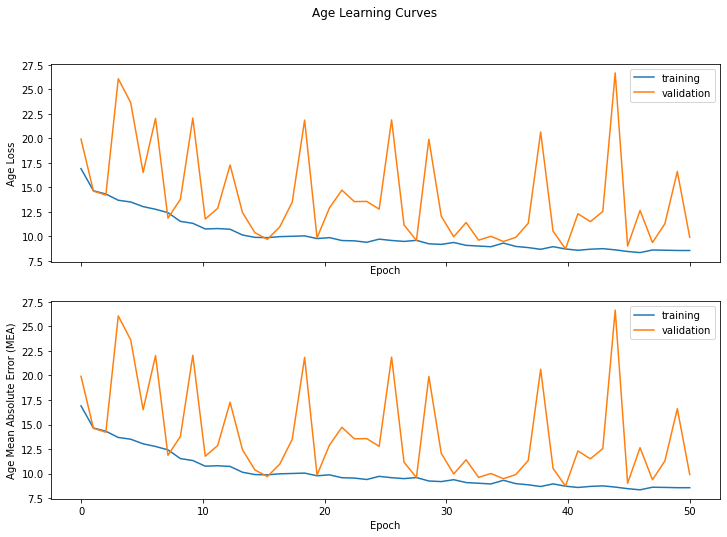
\includegraphics[height=0.42\textheight]{ModelA_AgeLearning_FCNDropout_GenderGreyScale_NoRegularisation.png}
    \label{fig:modelA_gs_gender_age_lc}
\end{figure}
\begin{figure}[h!]
    \centering
    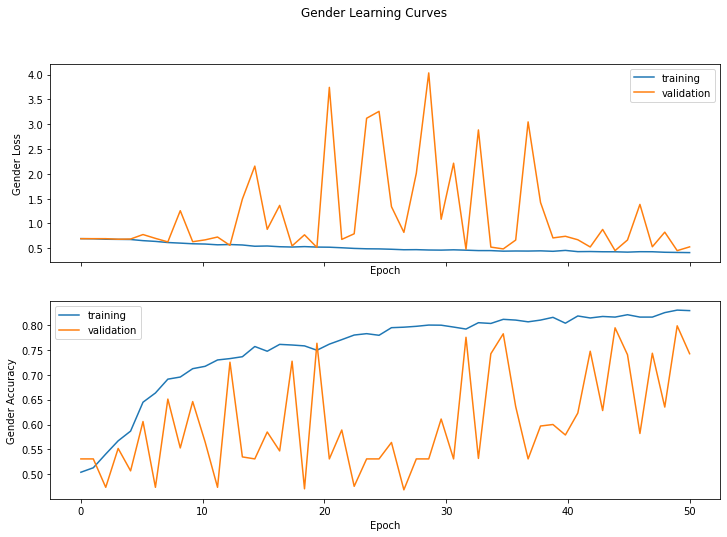
\includegraphics[height=0.42\textheight]{ModelA_GenderLearning_FCNDropout_GenderGreyScale_NoRegularisation.png}
    \label{fig:modelA_gs_age_age_lc}
\end{figure}
\newpage

\section{Old Model A Graph}
\begin{figure}[h!]
    \centering
    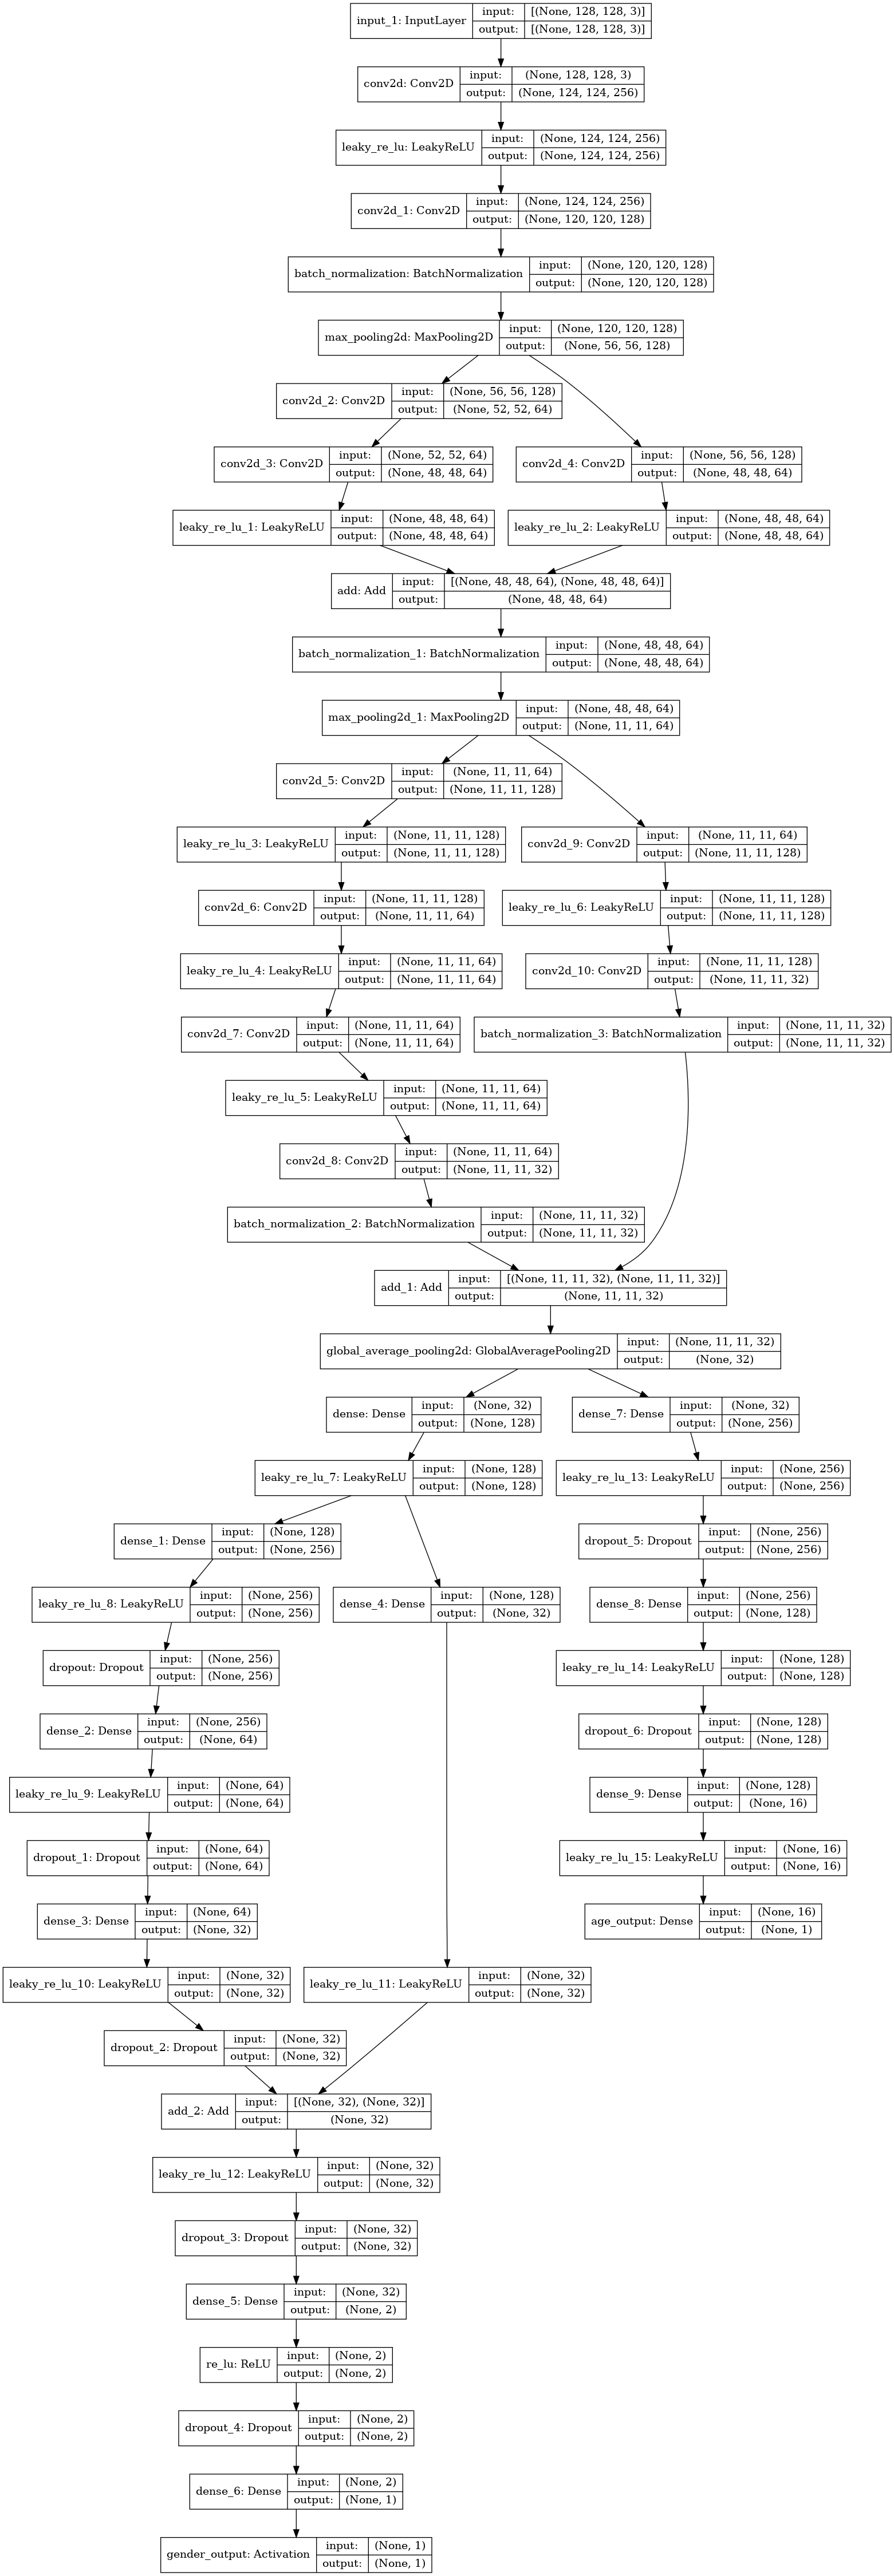
\includegraphics[height=0.9\textheight]{ModelAGraph_sample.png}
    \label{fig:modelA_original_graph_gs_neither}
\end{figure}
\newpage

\section{Model A Hyper-Parameter Tuning} \label{appendix:Model_A_Hyper-Parameter_Tuning}
\begin{figure}[h!]
    \centering
    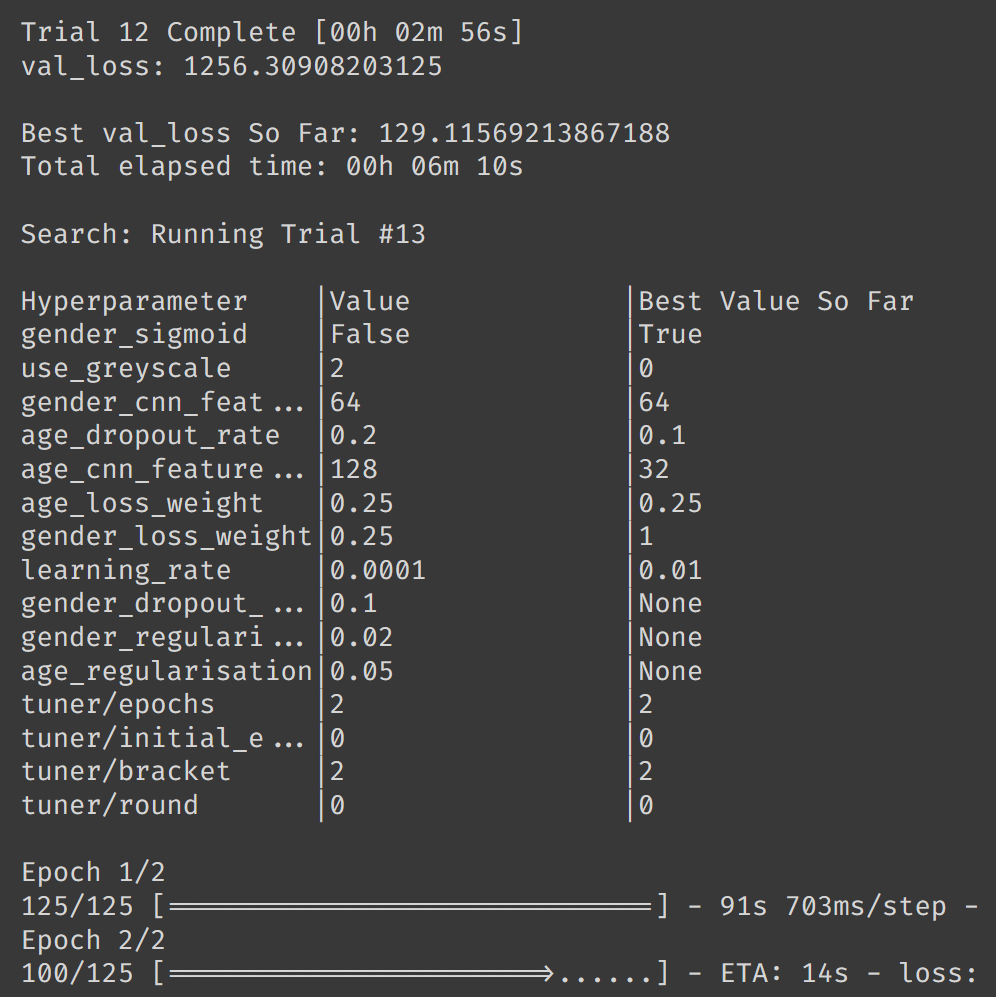
\includegraphics[height=0.9\textheight]{HyperParameter_Tuning.png}
    \label{fig:modelA_hyperparam_tuning}
\end{figure}

\section{Model B Epoch Traces}
\subsection{Epoch With Best Weights}\label{appendix:modelB_best_epoch}
\begin{verbatim}
Epoch 25/50
125/125 [==============================] - 37s 295ms/step 
- loss: 137.7862 
- age_output_loss: 85.8010 
- gender_output_loss: 0.1336 
- age_output_mean_absolute_error: 6.6296 
- gender_output_binary_accuracy: 0.9495 
- val_loss: 148.9740 
- val_age_output_loss: 84.2459 
- val_gender_output_loss: 0.2754 
- val_age_output_mean_absolute_error: 6.4352 
- val_gender_output_binary_accuracy: 0.8952
\end{verbatim}
\subsection{Early Stopping Epochs}\label{appendix:modelB_early_stopping_epochs}
\begin{verbatim}
    Epoch 25/50 
    125/125 [==============================] - 37s 295ms/step - loss: 137.7862 - age_output_loss: 85.8010 - gender_output_loss: 0.1336 - age_output_mean_absolute_error: 6.6296 - gender_output_binary_accuracy: 0.9495 - val_loss: 148.9740 - val_age_output_loss: 84.2459 - val_gender_output_loss: 0.2754 - val_age_output_mean_absolute_error: 6.4352 - val_gender_output_binary_accuracy: 0.8952
    Epoch 26/50
    125/125 [==============================] - 37s 293ms/step - loss: 132.8992 - age_output_loss: 81.6965 - gender_output_loss: 0.1276 - age_output_mean_absolute_error: 6.4587 - gender_output_binary_accuracy: 0.9545 - val_loss: 170.6825 - val_age_output_loss: 112.0731 - val_gender_output_loss: 0.3048 - val_age_output_mean_absolute_error: 7.3826 - val_gender_output_binary_accuracy: 0.8861
    Epoch 27/50
    125/125 [==============================] - 36s 290ms/step - loss: 132.8922 - age_output_loss: 81.7933 - gender_output_loss: 0.1241 - age_output_mean_absolute_error: 6.5250 - gender_output_binary_accuracy: 0.9540 - val_loss: 184.4266 - val_age_output_loss: 112.8646 - val_gender_output_loss: 0.4228 - val_age_output_mean_absolute_error: 7.1937 - val_gender_output_binary_accuracy: 0.8427
    Epoch 28/50
    125/125 [==============================] - 37s 292ms/step - loss: 127.1637 - age_output_loss: 76.9677 - gender_output_loss: 0.1166 - age_output_mean_absolute_error: 6.3486 - gender_output_binary_accuracy: 0.9545 - val_loss: 162.6561 - val_age_output_loss: 95.7592 - val_gender_output_loss: 0.3453 - val_age_output_mean_absolute_error: 6.9558 - val_gender_output_binary_accuracy: 0.8780
    Epoch 29/50
    125/125 [==============================] - 36s 290ms/step - loss: 127.2952 - age_output_loss: 78.4763 - gender_output_loss: 0.1051 - age_output_mean_absolute_error: 6.3871 - gender_output_binary_accuracy: 0.9590 - val_loss: 150.4551 - val_age_output_loss: 79.4326 - val_gender_output_loss: 0.3301 - val_age_output_mean_absolute_error: 6.3020 - val_gender_output_binary_accuracy: 0.8810
    Epoch 30/50
    125/125 [==============================] - 37s 294ms/step - loss: 127.9663 - age_output_loss: 78.2092 - gender_output_loss: 0.1136 - age_output_mean_absolute_error: 6.3384 - gender_output_binary_accuracy: 0.9595 - val_loss: 169.1610 - val_age_output_loss: 107.0598 - val_gender_output_loss: 0.3352 - val_age_output_mean_absolute_error: 7.1232 - val_gender_output_binary_accuracy: 0.8851
\end{verbatim}
